\section{Application to Compressive Sensing}
\subsection{Introduction}
\paragraph{Prior Work}
\subsection{Method}
\paragraph{Compressive Sensing} In many applications we can not observe $x(t)$ in real time. Instead, we observe $p$ detectors, and each detector provides a linear combination of a small number of coordinates of $x(t)$ at a time:
\begin{equation}
    \label{eq:cs_definition}
    y(t) = A_t x(t), \quad A_t \in \mathbb{R}^{p\times n}
\end{equation}

In particular, we consider a single pixel camera setup where for every time instance $t$, $p$ acquisitions $y(t)$ are obtained by a high sampling rate photo-detector using the projection matrix $A_t$. The rows of the matrix $A_t$ correspond to a binary mask pattern that can be encoded using a digital micro-mirror device (DMD) where the incoming light from $x(t)$ is reflected from the DMD array and focused onto the photo-detector. Figure~\ref{fig:SPI} illustrates an example of the single pixel imaging setup where a gas plume is imaged using a DMD array and a medium infra-red (MIR) photo-detector. 
\begin{figure}
\centering
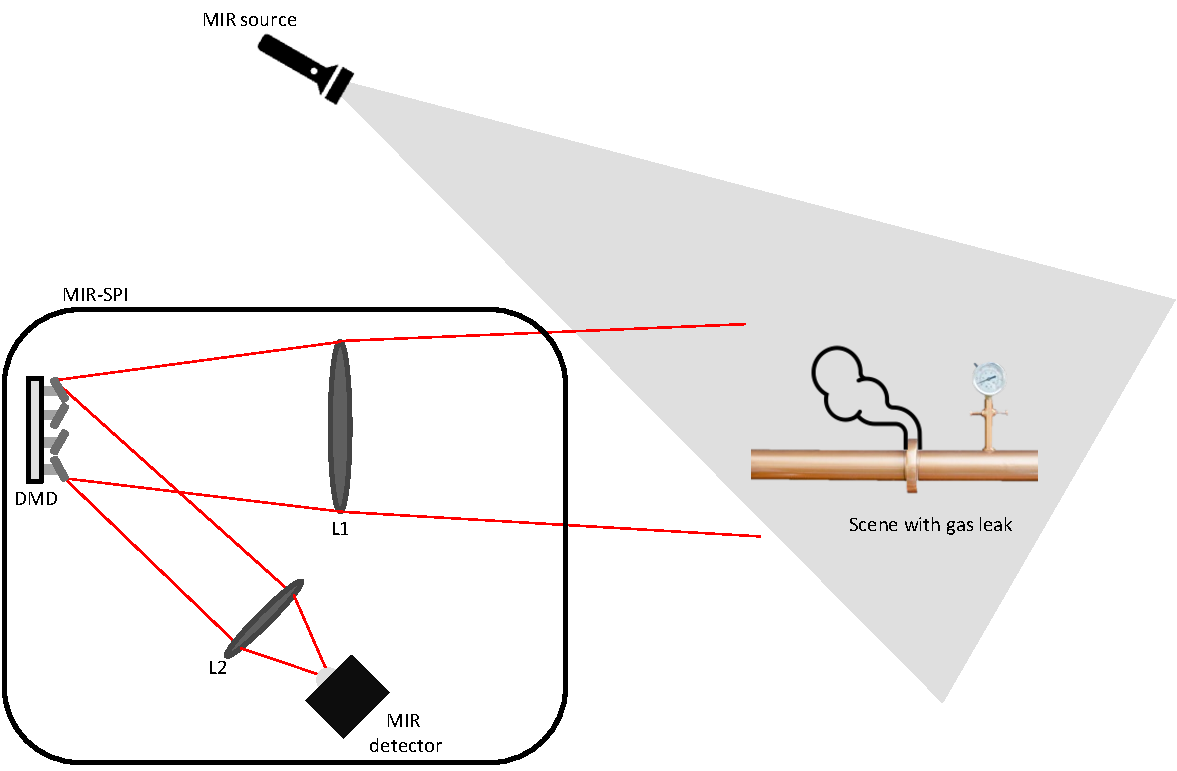
\includegraphics[width = 0.5\textwidth]{figures/SPI_setup.pdf}\label{fig:SPI}
\end{figure}

However, it is often possible to have access to a complete state $x(t)$ at the moment of model training. Thus, one can develop a ROM $(\psi_\theta, \phi_\theta, h_\theta)$ using the full state $x(t)$, and then utilize this ROM for real-time compressive sensing applications. 

\paragraph{Training Loss} Similar to prior works \cite{takeishi2017learning,morton2019deep,gin2021deep}, we define a \textit{data-driven loss} $\LL_{data}$ as a sum of reconstruction and prediction losses. The former ensures that $\phi_\theta$ and $\psi_\theta$ are inverse mappings of each other, whereas the latter matches the model's predictions to the available data. Formally, for a given set of trajectories $\bd{x}_i$, $i \in [1 \dots k]$, where each trajectory $\bd{x}_i \in \mathbb{R}^{n \times p}$ is a set of $p$ snapshots that correspond to the recorded states of the system for $p$ time-steps, $t_j$, $j \in [1, \dots, p]$, the loss function $\LL^{data}_\theta$ is defined as:

\begin{align}
    \label{eq:loss_training}
    \LL^{training}(\theta) & = \frac{1}{2\sigma^2}\sum_{i = 1}^k \left[\frac{\omega_1}{p}\sum_{j=1}^p\left\|\bd{x_i}(t_j) - \psi_\theta(\phi_\theta(\bd{x_i}(t_j)))\right\|^2\right. + \\
     & + \left.\frac{\omega_2}{p}\sum_{j=1}^p \left\|\psi_\theta\left(\phi_\theta(\bd{x_i}(t_1)) + \int_{t_1}^{t_j}h(z(t))dt\right) - \bd{x_i}(t_j)\right\|^2 \right]
\end{align}
where $\sigma$ is the standard deviation of the observation noise.

To obtain a ROM $(\psi_{\theta^*}, \phi_{\theta^*}, h_{\theta^*})$, we minimize the loss above:

\begin{equation}
    \label{eq:training_minimization}
    \theta^* = \arg\min_{\theta} \LL^{training}(\theta)
\end{equation}

We note that each trajectory $\bd{x}_i$ may be captured over its own time-frame and use a distinct, possibly non-uniform, step-size, in which case the loss function should be modified accordingly\footnote{The implementation is affected only in evaluating the integral in~(\ref{eq:loss_data_driven}). This part is handled by \texttt{torchdiffeq}~\cite{chen2018neural} library, which supports non-uniform time-frames within a batch}. To simplify the notation without loss of generality, in the rest of the paper we assume that all trajectories were recorded over the same time-frame with an equal and uniform step-size. 

\paragraph{Reconstruction Loss} 
We use the ROM $(\psi_{\theta^*}, \phi_{\theta^*}, h_{\theta^*})$ above to forecast the dynamics based on partial observations in real time. Namely, instead of reconstructing $x(t)$ based on compressive-sensing observations $y(t)$ directly, we first reconstruct the latent dynamics $z(t)$ and then project it to the observable space using the decoder $\psi_{\theta^*}(z)$.

\begin{align}
    \label{eq:reconstruction_problem_differential}
    \min_{\{z_t\}_{t=1, \dots, T}} & \frac{1}{2}\sum_{t=1}^T \left\|y_t - A\psi_{\theta^*}(z_t)\right\|_2^2 \\
    \text{s.t. } & \dot{z} = h_{\theta^*}(z)
\end{align}

We integrate the constraint and write it in its Lagrangian form:
\begin{align}
\label{eq:reconstruction_problem_integral}
    \min_{\{z_t\}_{t=1, \dots, T}} \LL_{\theta^*}^{recon}(z)
\end{align}

where 

\begin{equation}
    \label{eq:reconstruction_loss}
     \LL_{\theta^*}^{recon}(z) = \frac{1}{2}\sum_{t=1}^T \left\|y_t - A\psi_{\theta^*}(z_t)\right\|_2^2 + \frac{\lambda}{2} \sum_{t=1}^T \left\|z_{t-1} + \int_{t-1}^{t}h_{\theta^*}(z)dz - z_t\right\|_2^2
\end{equation}

where the parameter $\lambda$ controls the degree on which the compressing sensing algorithm relies on the latent dynamics $h_{\theta^*}$ during the signal reconstruction phase. We minimize the loss~\ref{eq:reconstruction_loss} using a gradient-based technique, with the gradients obtained using automatic differentiation frameworks. 

\subsection{Experiments}
\subsection{Discussion and Conclusion}
